\section{Inbetriebnahme}
    Zum Ausführen des Spiels muss zuerst die Assemblerdatei in einer IDE wie z.B. Geany (Freeware: \url{https://www.geany.org/}) geöffnet werden (rote Markierung, Abbildung \ref{fig:geany}).
    \begin{figure}[H]
        \centering
        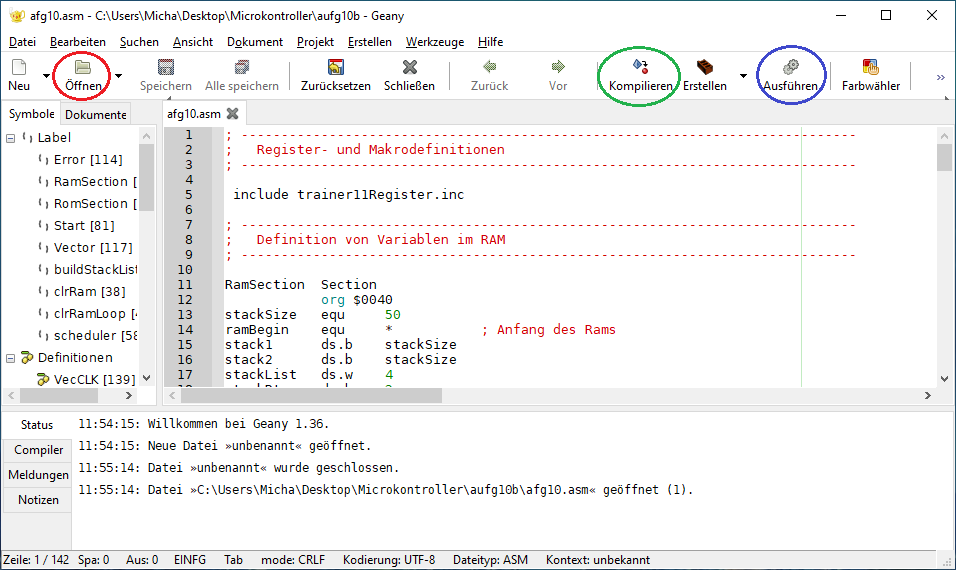
\includegraphics[scale=0.5]{img/geany.png}    
        \caption{Geany IDE}
        \label{fig:geany}
    \end{figure}
    Als nächstes müssen die Einstellungen in Geany geändert werden: 
    Zunächst der verwendete Kompiler, welchen wir von miniIDE nutzen, welche vorher im Verzeichnis \texttt{C:\textbackslash{}miniide} installiert sein muss (ansonsten muss der Pfad zum Kompiler später entsprechend angepasst werden).
    Ebenfalls benötigt wird die Software \textit{Realterm} in dem Verzeichnis \texttt{C:\textbackslash{}realterm}.
    \\
    Unter dem Stichwort \textit{Dokument} \textrightarrow{} \textit{Dateityp festlegen} \textrightarrow{} \textit{Kompilersprachen} muss \textit{Assembler} ausgewählt werden,
    danach im Menü-band unter \textit{Erstellen} erreicht man den Punkt \textit{Kommandos zum Erstellen konfigurieren} (Abbildung \ref{fig:geany-menu}).
    \begin{figure}[H]
        \centering
        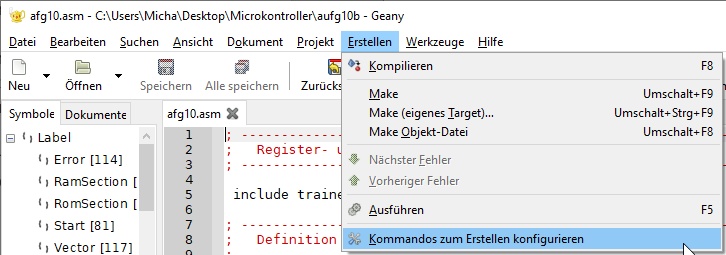
\includegraphics[scale=0.5]{img/geany-menu.png}    
        \caption{Geany IDE Menü}
        \label{fig:geany-menu}
    \end{figure}
    Hier muss nun unter \textit{Kommandos für ASM} folgendes eingetragen werden:
    \begin{center}
        \texttt{C:\textbackslash{}miniIDE\textbackslash{}ASM11 \%f -l}
    \end{center}
    und unter \textit{Befehle zum Ausführen}:
    \begin{center}
        \texttt{C:\textbackslash{}Realterm\textbackslash{}realterm "{}first"{} "{}display=1"{} "{}rows=40"{} "{}baud=9600"{} "{}sendfile=\%d\textbackslash{}\%e.s19"{}}
    \end{center}
    \begin{figure}[H]
        \centering
        \label{geany-config}
        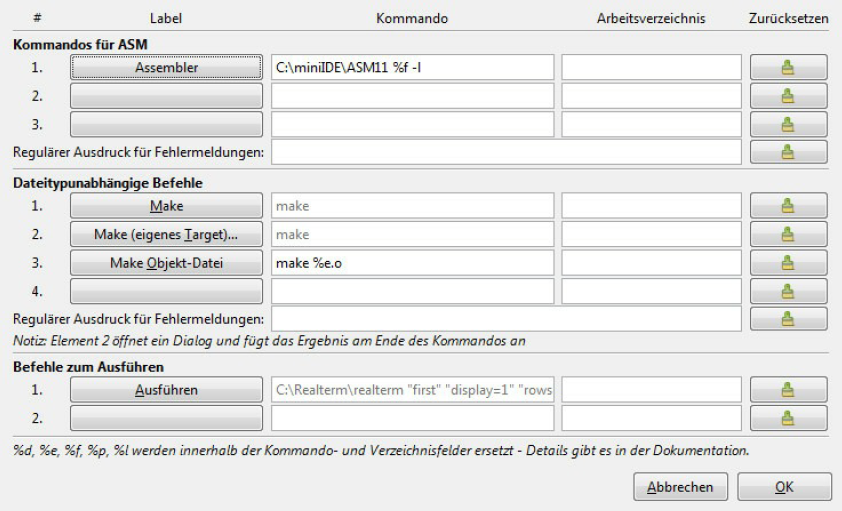
\includegraphics[scale=0.5]{img/geany-config.png}    
        \caption{Geany IDE Konfiguration}
    \end{figure}
    Gegebenenfalls muss hier noch \textit{Port=} mit der Nummer des entsprechenden COM-Ports ergänzt werden.
    \\
    Nach dem bestätigen per \textit{OK} müssen die Daten kompiliert und auf das Board überspielt werden (grüne und blaue Markierungen, Abbildung \ref{fig:geany}).
    Nach dem Klick auf \textit{Ausführen} öffnet sich jetzt \textit{Realterm} (Abbildung \ref{fig:realterm}). Nach betätigung des Resetschalters können die Daten mit 
    \textit{Send File}, im Reiter \textit{Send}, ans Board übertragen werden. 
    \begin{figure}[H]
        \centering
        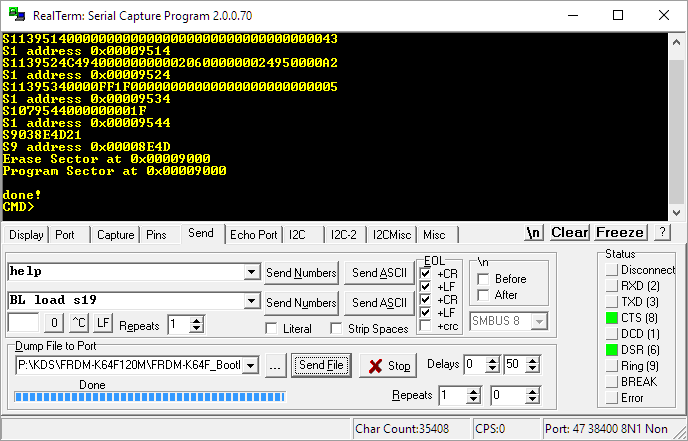
\includegraphics[scale=0.5]{img/realterm.png}    
        \caption{Realterm}
        \label{fig:realterm}
    \end{figure}

